\documentclass[a4paper,11pt,twoside,openright]{book} % Type du document

% compiler avec: pdflatex, bibtex, pdflatex, pdflatex
% require Pygmentize

% to install Pygmentize on macOS:
% brew install python
% pip3 install pygments
% sudo ln -s "$(which pygmentize)" /Library/TeX/texbin/pygmentize

% +---------------------------------------------------------------+
% | Language
% +---------------------------------------------------------------+
\usepackage[T1]{fontenc}
\usepackage[utf8]{inputenc}
\usepackage[french]{babel}

\newif\ifisconfidential	\isconfidentialfalse

\newif\ifisdraft\isdraftfalse



% +---------------------------------------------------------------+
% | Paramètres
% +---------------------------------------------------------------+

\newcommand{\TBtitle}{Titre du TB}
\newcommand{\TBsubtitle}{Sous-titre}%laisser vide si pas de sous-titre
\newcommand{\TByear}{2024}
\newcommand{\TBacademicYears}{2023-24}

\newcommand{\TBdpt}{Département des Technologie de l'information et de la communication (TIC)}
\newcommand{\TBfiliere}{Filière <<Informatique et systèmes de communication>>}
\newcommand{\TBorient}{Orientation <<Sécurité informatique>>}

\newcommand{\TBauthor}{EtuPrenom EtuNom}
\newcommand{\TBsupervisor}{Prof. Bli Bla}
\newcommand{\TBindustryContact}{Nom}
\newcommand{\TBindustryName}{EntrepriseZ}
\newcommand{\TBindustryAddress}{%
  Rue XY\\
  1400 Yverdon-les-Bains
}

% Confidentiel?
% uncomment if confidential / comment if not confiential
% \isconfidentialtrue

\newcommand{\TBresumePubliable}{
Dans ce travail... Ceci est le résumé publiable...
}

% +---------------------------------------------------------------+



% +-[set path]-------------------------------------+
\usepackage{template/TB-style}
\usepackage{template/TB-macros}
\usepackage{template/TB-template}
%\graphicspath{images/}
\usepackage{hyperref} %Doit etre le dernier package
\usepackage{pgfgantt} %for Gantt

\begin{document}

\frontmatter
\pagestyle{empty}

% TITLE and template
% +---------------------------------------------------------------+

\TBmaketitle

\pagestyle{frontmatter}

\TBsecondTitle

\TBpreambule

\TBauthentification


% Cahier des charges
% +---------------------------------------------------------------+
\chapter{Cahier des charges}



\section*{Résumé du problème}
%exemple
\lipsum[110-111]

\subsection*{Problématique}
%exemple
\lipsum[110-110]

\subsection*{Solutions existantes}
%exemple
\lipsum[1-1]

\subsection*{Solutions possibles}
%exemple
\lipsum[1-1]



\section*{Cahier des charges}
%exemple
\lipsum[1-1]


\subsection*{Objectifs}
%exemple
\lipsum[1-1]

\subsection*{Déroulement}
Le travail commence le ... et se termine le .... Sur les 16 premières semaines, soit du x au y, la charge de travail représente 12h par semaine. Les 6 dernières semaines, soit du x au y, ce travail sera réalisé à plein temps.

Un rendu intermédiaire noté est demandé le x et le rendu final est prévu pour le x à 12h00. 

La défense sera organisée entre le x et le y.

\subsection*{Livrables}
Les délivrables seront les suivants :
\begin{enumerate}
\item Une documentation contenant :
	\begin{itemize}
	\item Une analyse de marché
	\item La décision qui découle de l’analyse
	\item Spécifications
	\item Les informations du module tel que le fonctionnement et les limitations 
	\item Une planification initiale et finale
	\item Un mode d’emploi
	\end{itemize}
\item Un module remplissant les objectifs défini au point 2.1.
\item Un software implémentant les améliorations s’il a été possible de les effectuer.
\end{enumerate}




% TOC
% +---------------------------------------------------------------+
\tableofcontents
\clearpage


% Content
% +---------------------------------------------------------------+

\mainmatter
\pagestyle{plain}

\chapter{Introduction}
\label{ch:intro}


%exemple
\lipsum[1-4]




\chapter{Planification}
\label{ch:planif}

\section{Planification initiale}
Un exemple de planification en latex. D'autres moyens sont possibles.

%exemple
\scalebox{0.6}{
\begin{ganttchart}[vgrid,
title/.style={fill=teal, draw=none},
title label font=\color{white}\bfseries,
title left shift=0,
title right shift=0,
%title top shift=0,
title height=.75,
group/.append style={draw=black, fill=black!50},
%group top shift=1,
bar/.append style={fill=gray!50},
%bar top shift=0,
%bar height=0.4,
%milestone top shift=0,
y unit chart=0.6cm,
x unit=0.6cm,
]{1}{28}
\gantttitle{Déroulement du projet}{28} \\
\gantttitlelist{1,...,28}{1} \\
%
\ganttgroup{Démarrage}{1}{5} \\
	\ganttbar{Kick-off meeting}{1}{1} \\
	\ganttbar{Documents administratifs (NDA, etc.)}{1}{2} \\
	\ganttbar[bar/.append style={fill=red!50}]{Analyse des besoins métiers}{2}{4} \\
	\ganttbar{Rédaction du cahier des charges}{2}{4} \\
%	
\ganttgroup{Réalisation de l'état de l'art}{3}{6} \\
	\ganttbar{Recherche des travaux}{3}{3} \\
	\ganttbar[bar/.append style={fill=red!50}]{Analyse du travail précédent}{4}{5} \\
	\ganttbar{Analyse de la techno X}{5}{6} \\
%	
\ganttgroup{Mise en place de l'environnement de dev}{5}{8} \\
	\ganttmilestone[milestone/.append style={fill=red!50}]{Liste des besoins}{5}{12} \\
	\ganttbar{Mise en place}{7}{8} \\
%
\ganttgroup{Développement}{9}{19} \\
	\ganttbar{Back-end}{9}{15} \\
	\ganttbar{Front-end}{14}{17} \\
	\ganttbar{Prod}{18}{19}\\
%
\ganttbar{Tests}{19}{21} \\
%
\ganttbar{Synthèse des résultats}{20}{22} \\
%
\ganttgroup{Documentation}{1}{22} \\
	\ganttmilestone[milestone/.append style={fill=red!50}]{Rapport intermédiaire}{12}{12} \\
	\ganttmilestone[milestone/.append style={fill=red!50}]{Rapport final}{22}{22} \\
	\ganttmilestone[milestone/.append style={fill=red!50}]{Défense}{28}{28} \\
%
\end{ganttchart}
}



\chapter{État de l'art}
\label{ch:etatdelart}


%exemple
\lipsum[1-4]



\chapter{Exemple de chapitre}

\lipsum[1]


\section{Rédiger des expressions mathématiques}

voici des maths intégrés : $3^2 / 4^3$.

ou alors à la ligne :

$$ \frac{3 x_a}{ y_b^2 +4}$$

\section{Insérer des images}

Voici comment mettre une image.

\begin{figure}
	\centering
	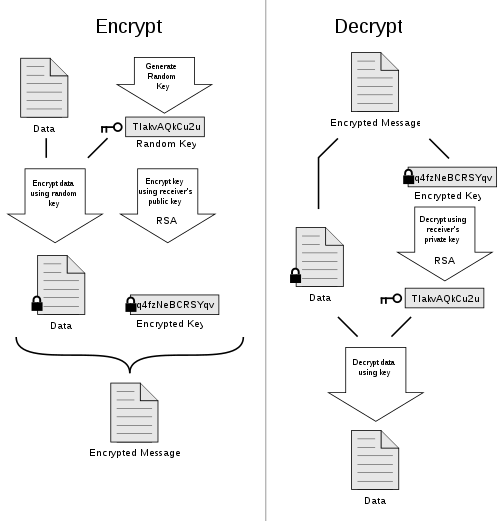
\includegraphics[width=8cm]{images/PGP_101.png}
	\caption{Schéma PGP}
	\label{fig:pgp}
\end{figure}


\section{Créer et citer une référence bibliographique}

Ceci est un exemple de citation d'un livre de Pasini~\cite{pasini2015}.

Mais aussi du site Web de Black Alps 2019~\cite{BA19} !


\section{Créer une référence à une autre partie de document}

On peut aussi ajouter une référence à la section~\ref{sec:shell}.

On peut aussi ajouter une référence à l'introduction, chapitre~\ref{ch:intro}.

Comme montre la Figure~\ref{fig:pgp}, on peut référencer une figure.


\section{Afficher une commande simple ou du bash}

Utiliser la commande \com{com}.

Exemple : Test d'une commande bash shell \com{ls} : 

Utiliser l'environnement \com{shellcmd}.

\begin{shellcmd}
$> ls -al test_underscore $$* "coucou"
\end{shellcmd}
Bli bLa


\section{Afficher une commande Shell}
\label{sec:shell}

Voici comment faire une mise en forme de commande SHELL.

Utiliser l'environnement \com{listingsbox}.
\begin{description}
 \item[1er paramètre:] le ype de shell, ici "console"
 \item[2ème paramètre:] le nom à donner à la box
\end{description}

\begin{listingsbox}{console}{Exemple de commande shell avec réponse}
root@kali:~$ bunzip2 data-decrypted.bin
bunzip2: Can't guess original name for data-decrypted.bin -- using
data-decrypted.bin.out
\end{listingsbox}


\section{Inclure du code dans le latex}

Utiliser l'environnement \com{sourcebox}.
\begin{description}
 \item[1er paramètre:] le ype de shell, ici "c"
 \item[2ème paramètre:] le nom à donner à la box
\end{description}

\begin{sourcebox}{c}{Exemple de code C}
#include <stdio.h>

int main(int argc, char* argv[])
{
   printf("Hello World!\n");
   return 0;
}
\end{sourcebox}



\section{Inclure du code à partir d'un fichier source externe}

Utiliser la commande \com{inputsourcecode}.
\begin{description}
 \item[1er paramètre:] le ype de shell, ici "c"
 \item[2ème paramètre:] le nom du fichier source, "\path{source_code/example.c}"\\ Egalement exemple de la commande \com{path}.
 \item[3ème paramètre:] le nom à donner à la box
\end{description}


%% Inclure du code source d'un fichier externe
%% 1er paramètre: langage du code
%% 2ème paramètre: le path du fichier source
%% 3ème paramètre: le titre de la box
\inputsourcecode{c}{"source_code/example.c"}{example.c}

Même exemple, mais en spécifiant les lignes 4 à 8 :
\inputsourcecode[firstline=4,lastline=8]{c}{"source_code/example.c"}{example.c}





\chapter{Architecture}
\label{ch:arch}


%exemple
\lipsum[1-4]



\chapter{Implementation}
\label{ch:impl}


%exemple
\lipsum[1-4]



\chapter{Conclusion}

%exemple
\lipsum[1-4]


% +---------------------------------------------------------------+
\cleardoublepage
\phantomsection
\addcontentsline{toc}{chapter}{Bibliographie}
\markboth{Bibliographie}{Bibliographie}
\bibliographystyle{plain}
\bibliography{chapters/biblio}
\nocite{*} %ajoute tout ce qu'il y a dans le bibtex

\phantomsection
\listoffigures
\addcontentsline{toc}{chapter}{Table des Figures}
\markboth{Table des Figures}{Table des Figures}

\phantomsection
\listoftables
\addcontentsline{toc}{chapter}{Liste des tableaux}
\markboth{Liste des tableaux}{Liste des tableaux}


% Annexes
% +---------------------------------------------------------------+
\appendix

\chapter{Outils utilisés pour la compilation}

%exemple
\lipsum[5-6]


\chapter{Journal de travail}

\begin{landscape}

\begin{longtable}[c]{lp{10cm}rrrr}
    \caption{Journal de travail}\\

    \hline
    Date & Description & Rech. [h] & Dev. [h] & Rapport [h] & Admin [h] \\
    \hline
    \endfirsthead
    
    \hline
    Date & Description & Rech. [h] & Dev. [h] & Rapport [h] & Admin [h] \\
    \hline
    \endhead
    
    \multicolumn{6}{r}{\small \it Le journal de travail continue à la page suivante.} \\
    \normalsize
    \endfoot
    
    \hline
    \endlastfoot


  % Work
	5.03.2020 
	& Kick-off meeting avec le mandant \lipsum[1-1]
	& 0 %recherche
	& 0 %dev
	& 0 %reporting
	& 2\\ %admin

	12.03.2020 
	& Recherche sur l'état de l'art
	& 4 %recherche
	& 0 %dev
	& 0 %reporting
	& 0\\ %admin

	19.03.2020 
	& Mise en place de l'environnement de développement et documentation
	& 0 %recherche
	& 7 %dev
	& 1 %reporting
	& 0\\ %admin

	25.03.2020 
	& Rédaction de l'état de l'art
	& 0 %recherche
	& 0 %dev
	& 4 %reporting
	& 0\\ %admin

	25.03.2020 
	& Dev de la partie interface
	& 0 %recherche
	& 0 %dev
	& 4 %reporting
	& 0\\ %admin
	
	
	xx.xx.2020 
	& Test
	& 0 %recherche
	& 0 %dev
	& 4 %reporting
	& 0\\ %admin
	
	xx.xx.2020 
	& Test
	& 0 %recherche
	& 0 %dev
	& 4 %reporting
	& 0\\ %admin

	xx.xx.2020 
	& Test
	& 0 %recherche
	& 0 %dev
	& 4 %reporting
	& 0\\ %admin

	xx.xx.2020 
	& Test
	& 0 %recherche
	& 0 %dev
	& 4 %reporting
	& 0\\ %admin

	xx.xx.2020 
	& Test
	& 0 %recherche
	& 0 %dev
	& 4 %reporting
	& 0\\ %admin

	xx.xx.2020 
	& Test
	& 0 %recherche
	& 0 %dev
	& 4 %reporting
	& 0\\ %admin
	
	xx.xx.2020 
	& Test
	& 0 %recherche
	& 0 %dev
	& 4 %reporting
	& 0\\ %admin

	xx.xx.2020 
	& Test
	& 0 %recherche
	& 0 %dev
	& 4 %reporting
	& 0\\ %admin

	xx.xx.2020 
	& Test
	& 0 %recherche
	& 0 %dev
	& 4 %reporting
	& 0\\ %admin

	xx.xx.2020 
	& Test
	& 0 %recherche
	& 0 %dev
	& 4 %reporting
	& 0\\ %admin
	
\end{longtable}


\end{landscape}



\end{document}
